% Figura: exemplo do PSP (instância A/0020, backlog, corredores e waves A, B e C) — gerada em TikZ
\documentclass[tikz,border=4pt]{standalone}
\usepackage[utf8]{inputenc}
\usepackage[T1]{fontenc}
\usepackage{times}
\usepackage{amsmath}
\usetikzlibrary{shapes.geometric}
\tikzset{
  caixa/.style={draw=black!70, line width=0.5pt, fill=white},
  sel/.style={draw=green!45!black, line width=1.4pt, fill=green!5},
  piso/.style={draw=black!60, line width=0.5pt},
  rotulo/.style={font=\small},
  titulo/.style={font=\normalsize},
}
% Item 0: círculo | Item 1: triângulo | Item 2: losango | Item 3: estrela | Item 4: cilindro
\newcommand{\shpa}[1]{\fill[blue!20,draw=blue!55] #1 circle (0.12);}
\newcommand{\shpb}[1]{\node[regular polygon,regular polygon sides=3,minimum size=0.34cm,inner sep=0pt,fill=red!25,draw=red!60] at #1 {};}
\newcommand{\shpc}[1]{\node[diamond,minimum size=0.30cm,inner sep=0pt,fill=yellow!40,draw=orange!70] at #1 {};}
\newcommand{\shpd}[1]{\node[star,star points=5,star point ratio=2.2,minimum size=0.32cm,inner sep=0pt,fill=violet!25,draw=violet!60] at #1 {};}
\newcommand{\shpe}[1]{\begin{scope}[shift={#1}]
  \filldraw[fill=green!25,draw=green!50!black] (-0.1,0.09) -- (-0.1,-0.09) arc[start angle=180,end angle=360,x radius=0.1,y radius=0.045] -- (0.1,0.09);
  \filldraw[fill=green!15,draw=green!50!black] (0,0.09) ellipse[x radius=0.1,y radius=0.045];
\end{scope}}
\begin{document}
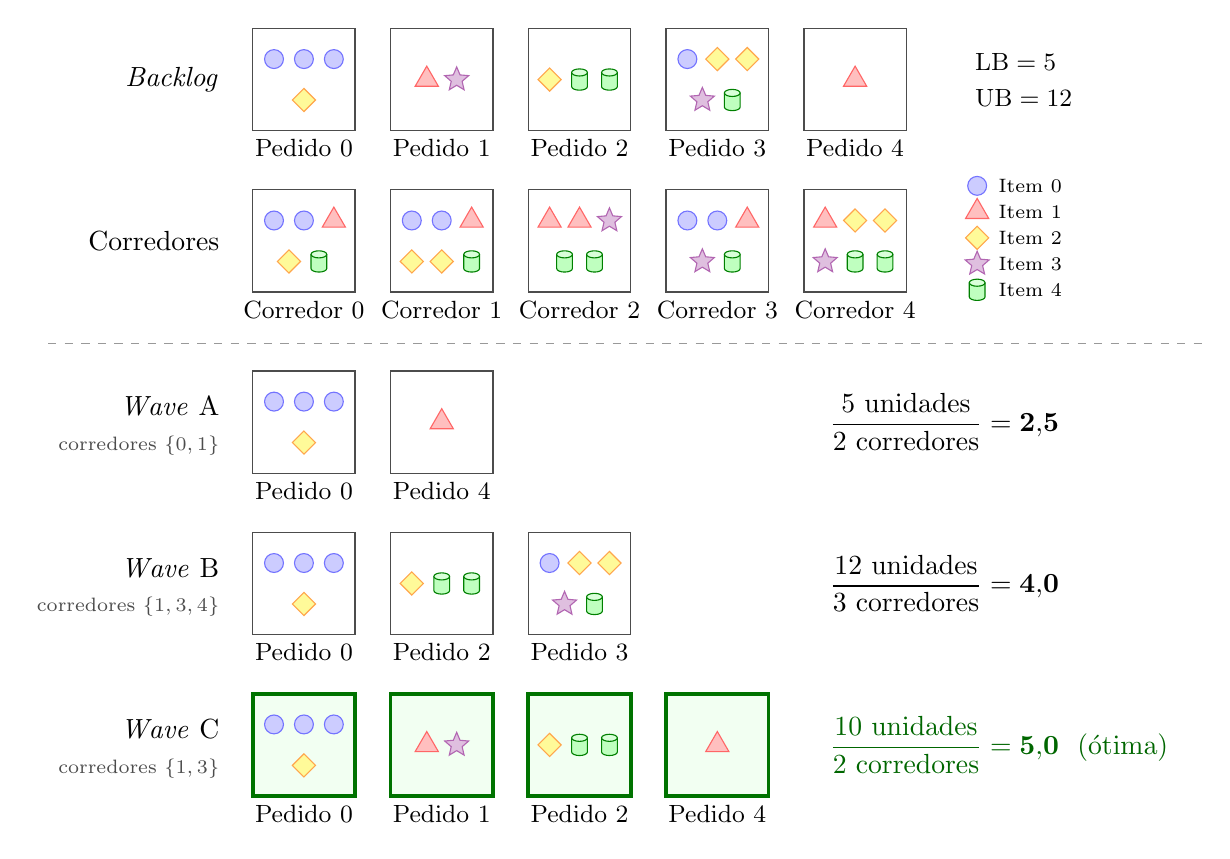
\begin{tikzpicture}
\node[titulo,anchor=east] at (2.3000000000000003,0.65) {\textit{Backlog}};
\draw[caixa] (2.6,0) rectangle ++(1.3,1.3);
\shpa{(2.870,0.910)}
\shpa{(3.250,0.910)}
\shpa{(3.630,0.910)}
\shpc{(3.250,0.390)}
\node[rotulo] at (3.25,-0.22) {Pedido 0};
\draw[caixa] (4.35,0) rectangle ++(1.3,1.3);
\shpb{(4.810,0.650)}
\shpd{(5.190,0.650)}
\node[rotulo] at (5.0,-0.22) {Pedido 1};
\draw[caixa] (6.1,0) rectangle ++(1.3,1.3);
\shpc{(6.370,0.650)}
\shpe{(6.750,0.650)}
\shpe{(7.130,0.650)}
\node[rotulo] at (6.75,-0.22) {Pedido 2};
\draw[caixa] (7.85,0) rectangle ++(1.3,1.3);
\shpa{(8.120,0.910)}
\shpc{(8.500,0.910)}
\shpc{(8.880,0.910)}
\shpd{(8.310,0.390)}
\shpe{(8.690,0.390)}
\node[rotulo] at (8.5,-0.22) {Pedido 3};
\draw[caixa] (9.6,0) rectangle ++(1.3,1.3);
\shpb{(10.250,0.650)}
\node[rotulo] at (10.25,-0.22) {Pedido 4};
\node[anchor=west,font=\small,align=left] at (11.65,0.65) {$\mathrm{LB} = 5$\\[2pt]$\mathrm{UB} = 12$};
\node[titulo,anchor=east] at (2.3000000000000003,-1.4) {Corredores};
\draw[caixa] (2.6,-2.05) rectangle ++(1.3,1.3);
\shpa{(2.870,-1.140)}
\shpa{(3.250,-1.140)}
\shpb{(3.630,-1.140)}
\shpc{(3.060,-1.660)}
\shpe{(3.440,-1.660)}
\node[rotulo] at (3.25,-2.27) {Corredor 0};
\draw[caixa] (4.35,-2.05) rectangle ++(1.3,1.3);
\shpa{(4.620,-1.140)}
\shpa{(5.000,-1.140)}
\shpb{(5.380,-1.140)}
\shpc{(4.620,-1.660)}
\shpc{(5.000,-1.660)}
\shpe{(5.380,-1.660)}
\node[rotulo] at (5.0,-2.27) {Corredor 1};
\draw[caixa] (6.1,-2.05) rectangle ++(1.3,1.3);
\shpb{(6.370,-1.140)}
\shpb{(6.750,-1.140)}
\shpd{(7.130,-1.140)}
\shpe{(6.560,-1.660)}
\shpe{(6.940,-1.660)}
\node[rotulo] at (6.75,-2.27) {Corredor 2};
\draw[caixa] (7.85,-2.05) rectangle ++(1.3,1.3);
\shpa{(8.120,-1.140)}
\shpa{(8.500,-1.140)}
\shpb{(8.880,-1.140)}
\shpd{(8.310,-1.660)}
\shpe{(8.690,-1.660)}
\node[rotulo] at (8.5,-2.27) {Corredor 3};
\draw[caixa] (9.6,-2.05) rectangle ++(1.3,1.3);
\shpb{(9.870,-1.140)}
\shpc{(10.250,-1.140)}
\shpc{(10.630,-1.140)}
\shpd{(9.870,-1.660)}
\shpe{(10.250,-1.660)}
\shpe{(10.630,-1.660)}
\node[rotulo] at (10.25,-2.27) {Corredor 4};
\shpa{(11.8,-0.700)}
\node[anchor=west,font=\scriptsize] at (11.950000000000001,-0.700) {Item 0};
\shpb{(11.8,-1.030)}
\node[anchor=west,font=\scriptsize] at (11.950000000000001,-1.030) {Item 1};
\shpc{(11.8,-1.360)}
\node[anchor=west,font=\scriptsize] at (11.950000000000001,-1.360) {Item 2};
\shpd{(11.8,-1.690)}
\node[anchor=west,font=\scriptsize] at (11.950000000000001,-1.690) {Item 3};
\shpe{(11.8,-2.020)}
\node[anchor=west,font=\scriptsize] at (11.950000000000001,-2.020) {Item 4};
\draw[black!40,dashed] (0,-2.6999999999999997) -- (14.65,-2.6999999999999997);
\node[titulo,anchor=east] at (2.3000000000000003,-3.4999999999999996) {\textit{Wave} A};
\node[font=\scriptsize,anchor=east,text=black!70] at (2.3000000000000003,-3.9999999999999996) {corredores $\{0,1\}$};
\draw[caixa] (2.6,-4.35) rectangle ++(1.3,1.3);
\shpa{(2.870,-3.440)}
\shpa{(3.250,-3.440)}
\shpa{(3.630,-3.440)}
\shpc{(3.250,-3.960)}
\node[rotulo] at (3.25,-4.569999999999999) {Pedido 0};
\draw[caixa] (4.35,-4.35) rectangle ++(1.3,1.3);
\shpb{(5.000,-3.700)}
\node[rotulo] at (5.0,-4.569999999999999) {Pedido 4};
\node[anchor=west,text=black] at (9.799999999999999,-3.6999999999999997) {$\dfrac{5\ \text{unidades}}{2\ \text{corredores}} = \mathbf{2{,}5}$};
\node[titulo,anchor=east] at (2.3000000000000003,-5.549999999999999) {\textit{Wave} B};
\node[font=\scriptsize,anchor=east,text=black!70] at (2.3000000000000003,-6.049999999999999) {corredores $\{1,3,4\}$};
\draw[caixa] (2.6,-6.3999999999999995) rectangle ++(1.3,1.3);
\shpa{(2.870,-5.490)}
\shpa{(3.250,-5.490)}
\shpa{(3.630,-5.490)}
\shpc{(3.250,-6.010)}
\node[rotulo] at (3.25,-6.619999999999999) {Pedido 0};
\draw[caixa] (4.35,-6.3999999999999995) rectangle ++(1.3,1.3);
\shpc{(4.620,-5.750)}
\shpe{(5.000,-5.750)}
\shpe{(5.380,-5.750)}
\node[rotulo] at (5.0,-6.619999999999999) {Pedido 2};
\draw[caixa] (6.1,-6.3999999999999995) rectangle ++(1.3,1.3);
\shpa{(6.370,-5.490)}
\shpc{(6.750,-5.490)}
\shpc{(7.130,-5.490)}
\shpd{(6.560,-6.010)}
\shpe{(6.940,-6.010)}
\node[rotulo] at (6.75,-6.619999999999999) {Pedido 3};
\node[anchor=west,text=black] at (9.799999999999999,-5.749999999999999) {$\dfrac{12\ \text{unidades}}{3\ \text{corredores}} = \mathbf{4{,}0}$};
\node[titulo,anchor=east] at (2.3000000000000003,-7.6) {\textit{Wave} C};
\node[font=\scriptsize,anchor=east,text=black!70] at (2.3000000000000003,-8.1) {corredores $\{1,3\}$};
\draw[caixa,sel] (2.6,-8.45) rectangle ++(1.3,1.3);
\shpa{(2.870,-7.540)}
\shpa{(3.250,-7.540)}
\shpa{(3.630,-7.540)}
\shpc{(3.250,-8.060)}
\node[rotulo] at (3.25,-8.67) {Pedido 0};
\draw[caixa,sel] (4.35,-8.45) rectangle ++(1.3,1.3);
\shpb{(4.810,-7.800)}
\shpd{(5.190,-7.800)}
\node[rotulo] at (5.0,-8.67) {Pedido 1};
\draw[caixa,sel] (6.1,-8.45) rectangle ++(1.3,1.3);
\shpc{(6.370,-7.800)}
\shpe{(6.750,-7.800)}
\shpe{(7.130,-7.800)}
\node[rotulo] at (6.75,-8.67) {Pedido 2};
\draw[caixa,sel] (7.85,-8.45) rectangle ++(1.3,1.3);
\shpb{(8.500,-7.800)}
\node[rotulo] at (8.5,-8.67) {Pedido 4};
\node[anchor=west,text=green!40!black] at (9.799999999999999,-7.799999999999999) {$\dfrac{10\ \text{unidades}}{2\ \text{corredores}} = \mathbf{5{,}0}$ \ (ótima)};
\end{tikzpicture}
\end{document}
